\documentclass{standalone}
\usepackage{tikz}
\begin{document}
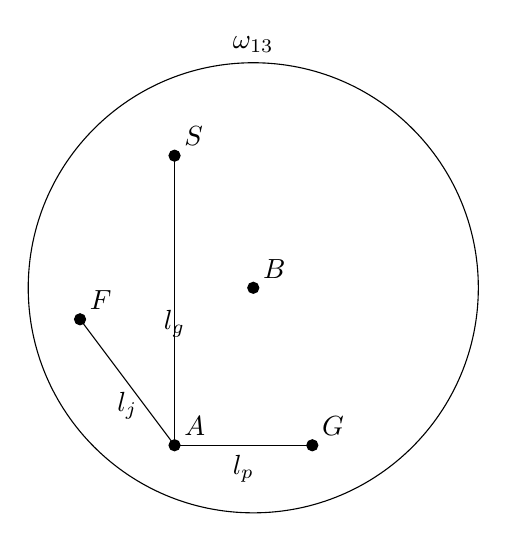
\begin{tikzpicture}[scale=1.0]
  \filldraw (0.0, 0.0) circle (2pt) node[above right] {$A$};
  \filldraw (1.7499, 0.0) circle (2pt) node[above right] {$G$};
  \filldraw (0.0, 3.6779) circle (2pt) node[above right] {$S$};
  \filldraw (-1.2, 1.6) circle (2pt) node[above right] {$F$};
  \filldraw (1.0, 2.0) circle (2pt) node[above right] {$B$};
  \draw (0.0, 0.0) -- (1.7499, 0.0) node[midway, below] {$l_p$};
  \draw (0.0, 0.0) -- (0.0, 3.6779) node[midway, below] {$l_g$};
  \draw (-1.2, 1.6) -- (0.0, 0.0) node[midway, below] {$l_j$};
  \draw (1.0, 2.0) circle (2.8582) node[above=2.8582cm] {$\omega_{13}$};
\end{tikzpicture}
\end{document}